%-----------------------------------
%-----------------------------------
% Beamer template made by Chenxiao
% 2023.11.04 at Qingdao,China
%-----------------------------------
%-----------------------------------

\documentclass{beamer}

\mode<presentation> {
	\usetheme{Madrid}
	\usecolortheme{rose}
	
	%\setbeamertemplate{footline}
	%若要删除所有幻灯片中的页脚,请取消注释此行
	
	%\setbeamertemplate{footline}[页码]
	%若要用简单的幻灯片计数替换所有幻灯片中的页脚,请取消注释此行
	
	%\setbeamertemplate{导航符号}{}
	%要删除所有幻灯片底部的导航符号,请取消注释此行
}

\usepackage{graphicx} % 允许包含图像
\usepackage{booktabs} % 允许在表中使用\toprule、\ midrule和\ bottomrule
\usepackage[UTF8,noindent]{ctexcap}  % 使用中文输入及显示
\usepackage[bookmarks=true]{hyperref}

%-----------------------------------
%	以下为正文
%-----------------------------------

\title[Paradigm: DDL]{Paradigm: DDL (Demo)} 
% 简短标题显示在每张幻灯片的底部,完整标题仅在标题页上

\author{骆沛荣 PB23010408} % Your name
\institute[数批] % 您的机构将出现在每张幻灯片的底部,可能是节省空间的简写
{
	Assignment D, C Programming Class (H) \\ % 你所在的机构
	\medskip
	 % Your email address
}
\date{\today} % 日期,可以更改为自定义日期

\begin{document}
	
	\begin{frame}
		\titlepage % 将标题页打印为第一张幻灯片
	\end{frame}
	
	\begin{frame}
		\frametitle{Overview} % 目录幻灯片,注释此块以将其删除
		\tableofcontents % 在整个演示过程中,如果您选择使用\ section{}和\ submission{}命令,这些命令将自动打印在此幻灯片上,作为演示的概述
	\end{frame}
	
	%-----------------------------------
	%	开始创建PPT
	%-----------------------------------
	
	\section{介绍} % 可以创建章节,以便将您的演讲组织成离散的块,所有章节和小节都会自动打印在目录中,作为演讲的概述
	
    \begin{frame}
    
        \sectionpage
    
    \end{frame}
	\begin{frame}
		\frametitle{你是否有如下困难……}
        \vfill
        \begin{itemize}[<+->]
            \item 今天的日程又没完成,怎么办?!?!\\\vfill
            \item 马上就要DDL了,报告赶不完了,怎么办?!?!\\\vfill
            \item \today 就要汇报$\mathbb D$题了,我的大作业才刚新建文件夹,怎么办?!?!\\\rightline{(一旁的舍友:啥大作业?不是教务系统吗?)}
        \end{itemize}
        \vfill
		\onslide<4>{\begin{center}
            \color{red}
            \textbf{不用担心,Paradigm: DDL来救你!}
            
        \end{center}}
	\end{frame}
	
	%------------------------------------------------
	
	\begin{frame}
		\frametitle{隆重推出}
        \begin{center}
            \begin{minipage}[l]{.3\textwidth}
                
\includegraphics[width=.9\textwidth]{launcher_icon.png}
            \end{minipage}
            \begin{minipage}[r]{.6\textwidth}
                \begin{Large}
                    \textbf{Paradigm: DDL\quad (Demo)}
                \end{Large}
                \medskip
                \\ \scriptsize{一款更适合(TODO:想个对象)的大作业管理软件}
            \end{minipage}
        \end{center}
		
        
	\end{frame}

    \begin{frame}
        \frametitle{简介}
        \vfill
        \begin{block}{项目概览}
        《Paradigm:DDL》是由我自己制作发行的一款大作业管理软件,于2023年11月底立项 ,原初测试于\today 开启,再临测试于未来开启,启程测试于未来开启,PC版技术性开放测试于未来开启,公测于未来开启。
        \end{block}
        \vfill
        \begin{block}{数据互通方面}
            在数据方面,同在没有官方服务器的情况下,iOS、PC、Android平台之间的账号数据目前还不能互通,玩家将来有可能可以在同一账号下切换设备。
        \end{block}
        \vfill
    \end{frame}

    \begin{frame}{简介}
        \vfill
        \begin{block}{技术简介}
            项目建立在一个被称作“Flutter
\includegraphics[width=1em]{ic_launcher.png}”的幻想世界,在这里,被神选中的人将被授予“Dart
\includegraphics[width=1em]{dart.png}”,导引跨平台之力。中间忘了——同时,逐步发掘“跨平台”的真相。
        \end{block}
        \vfill
        \begin{block}{Talk Is Cheap}
            
            \texttt{\href{https://github.com/Frigus27/Paradigm-DDL}{https://github.com/Frigus27/Paradigm-DDL}}
            {\par \scriptsize *代码过几天会上传。由于本人Flutter仅为初学水平,代码水平很烂,见谅)}
        \end{block}
        \vfill
    \end{frame}

    \section{Demo 演示}

    \begin{frame}
        \sectionpage
    \end{frame}
    \begin{frame}{界面预览(傳自我的手機)}
        \begin{center}
            \begin{minipage}[l]{.45\textwidth}
                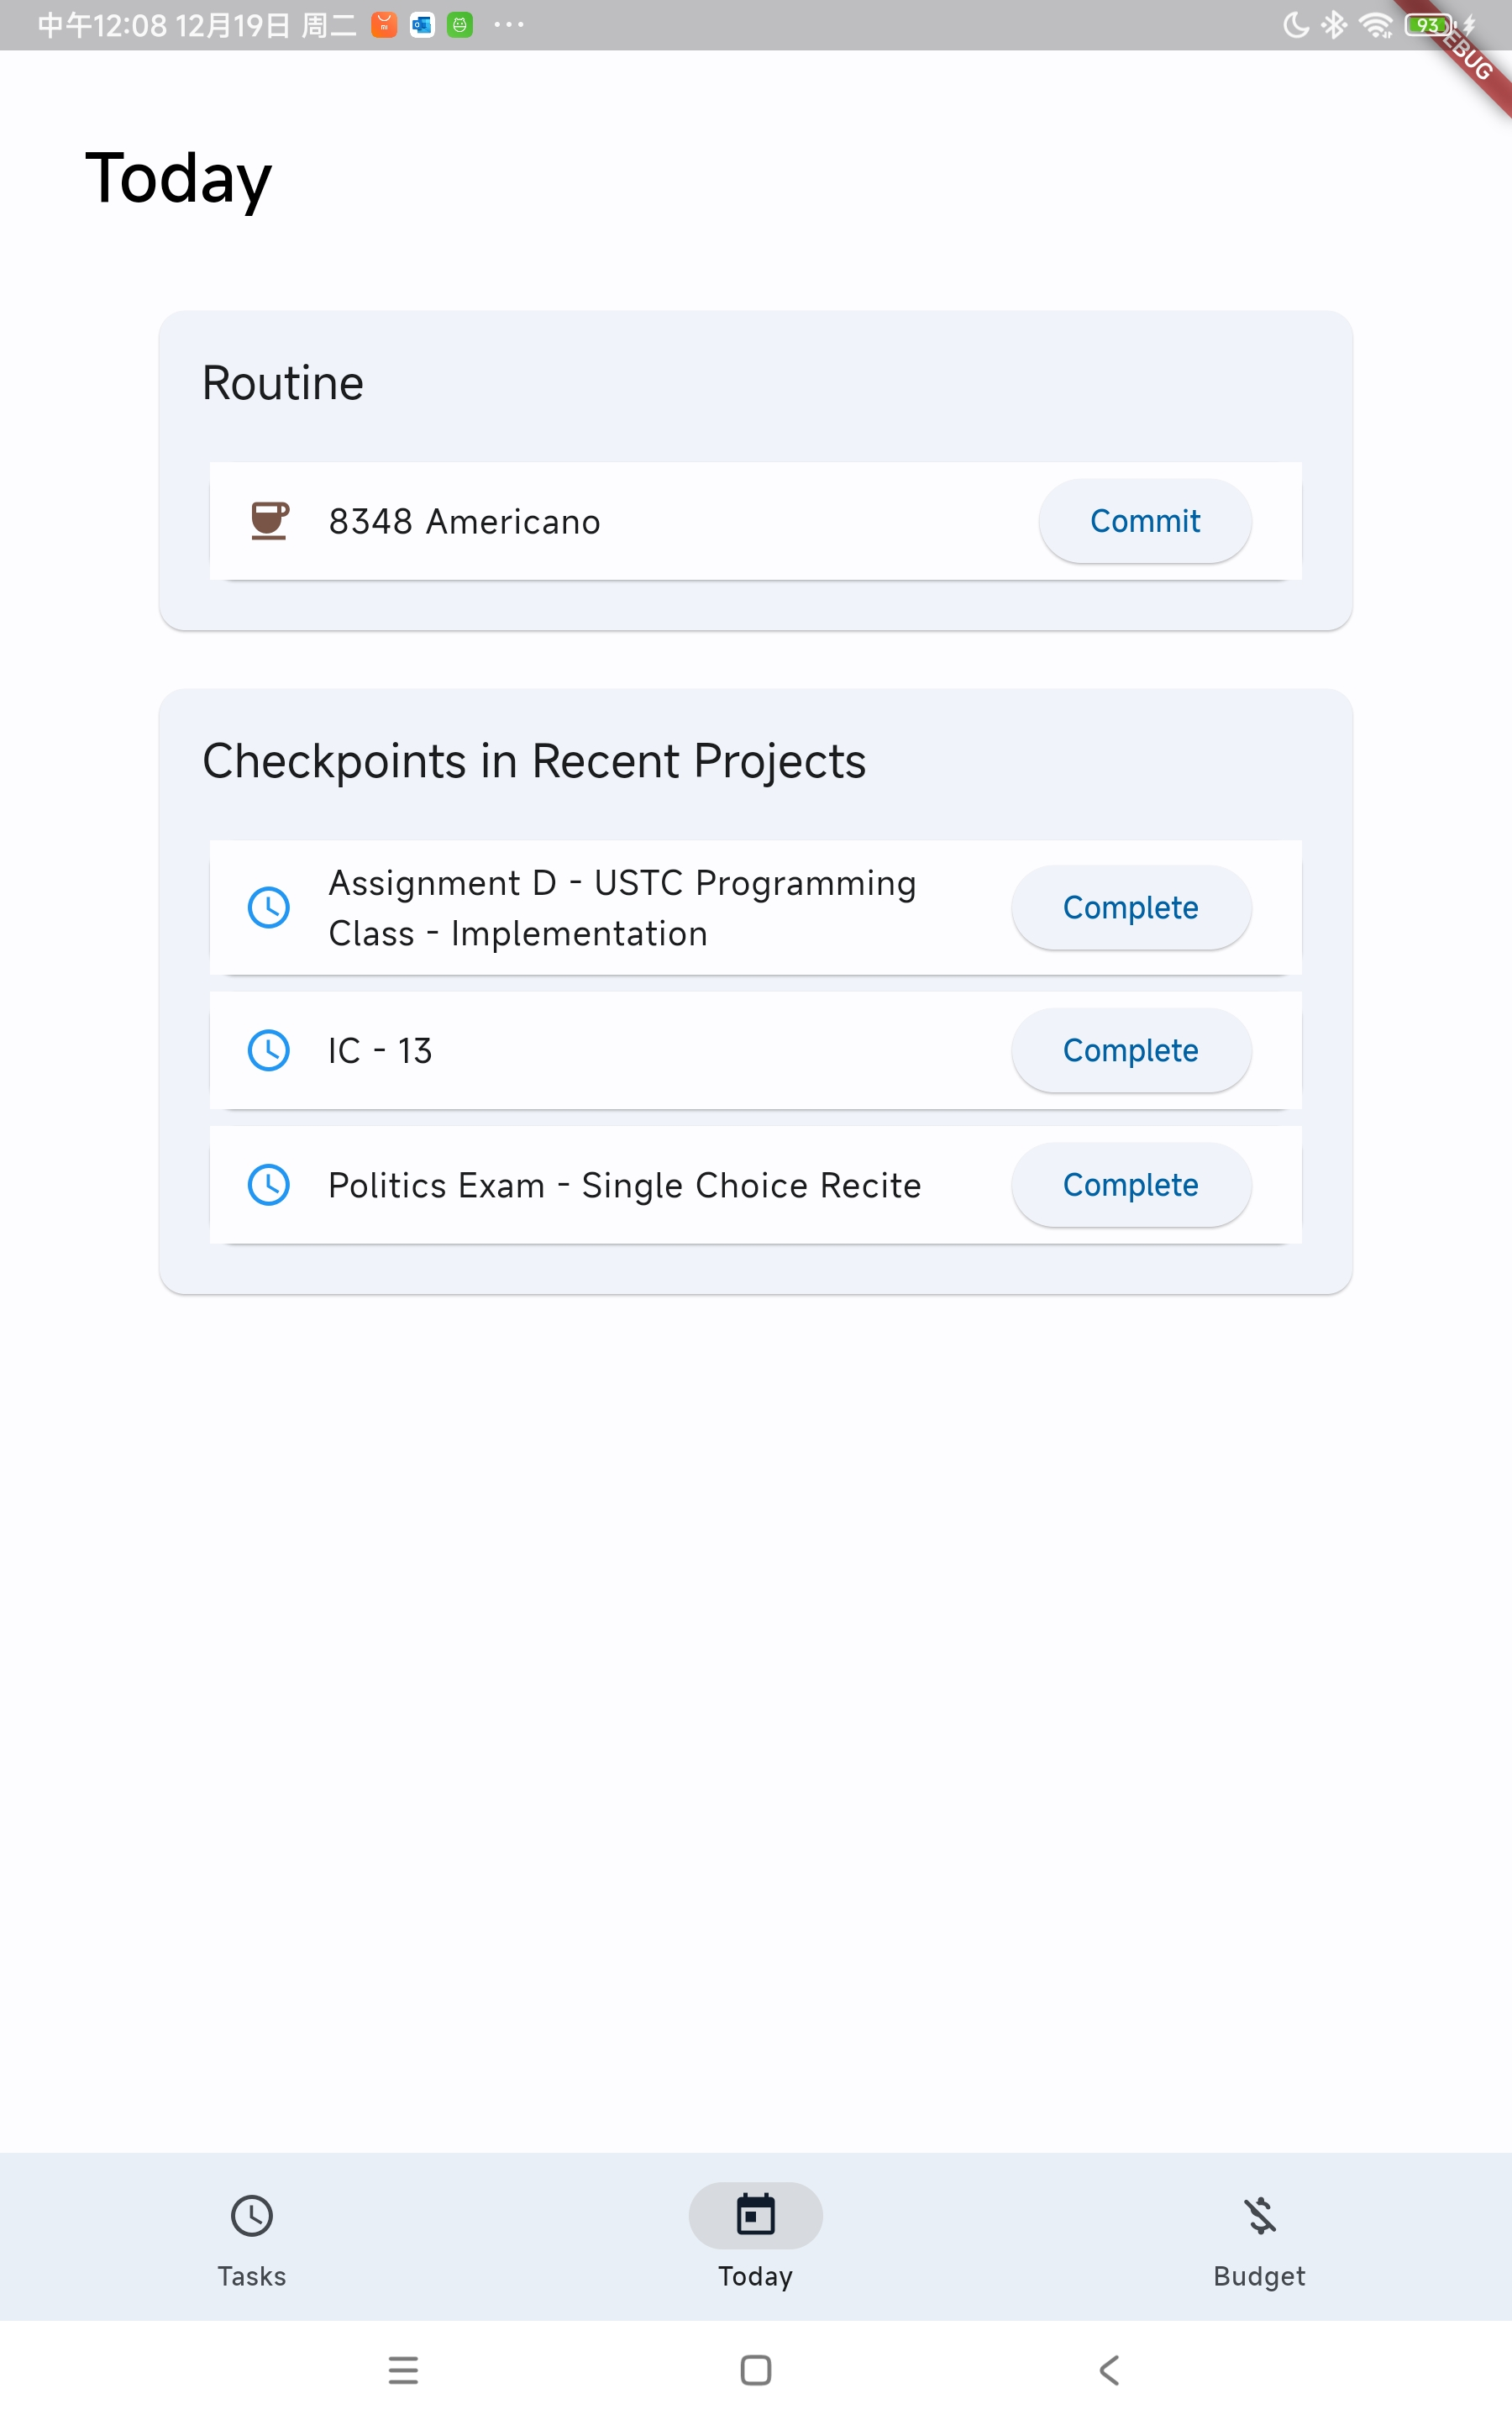
\includegraphics[width=.85\textwidth]{page-today.jpg}
            \end{minipage}
            \begin{minipage}[r]{.45\textwidth}
                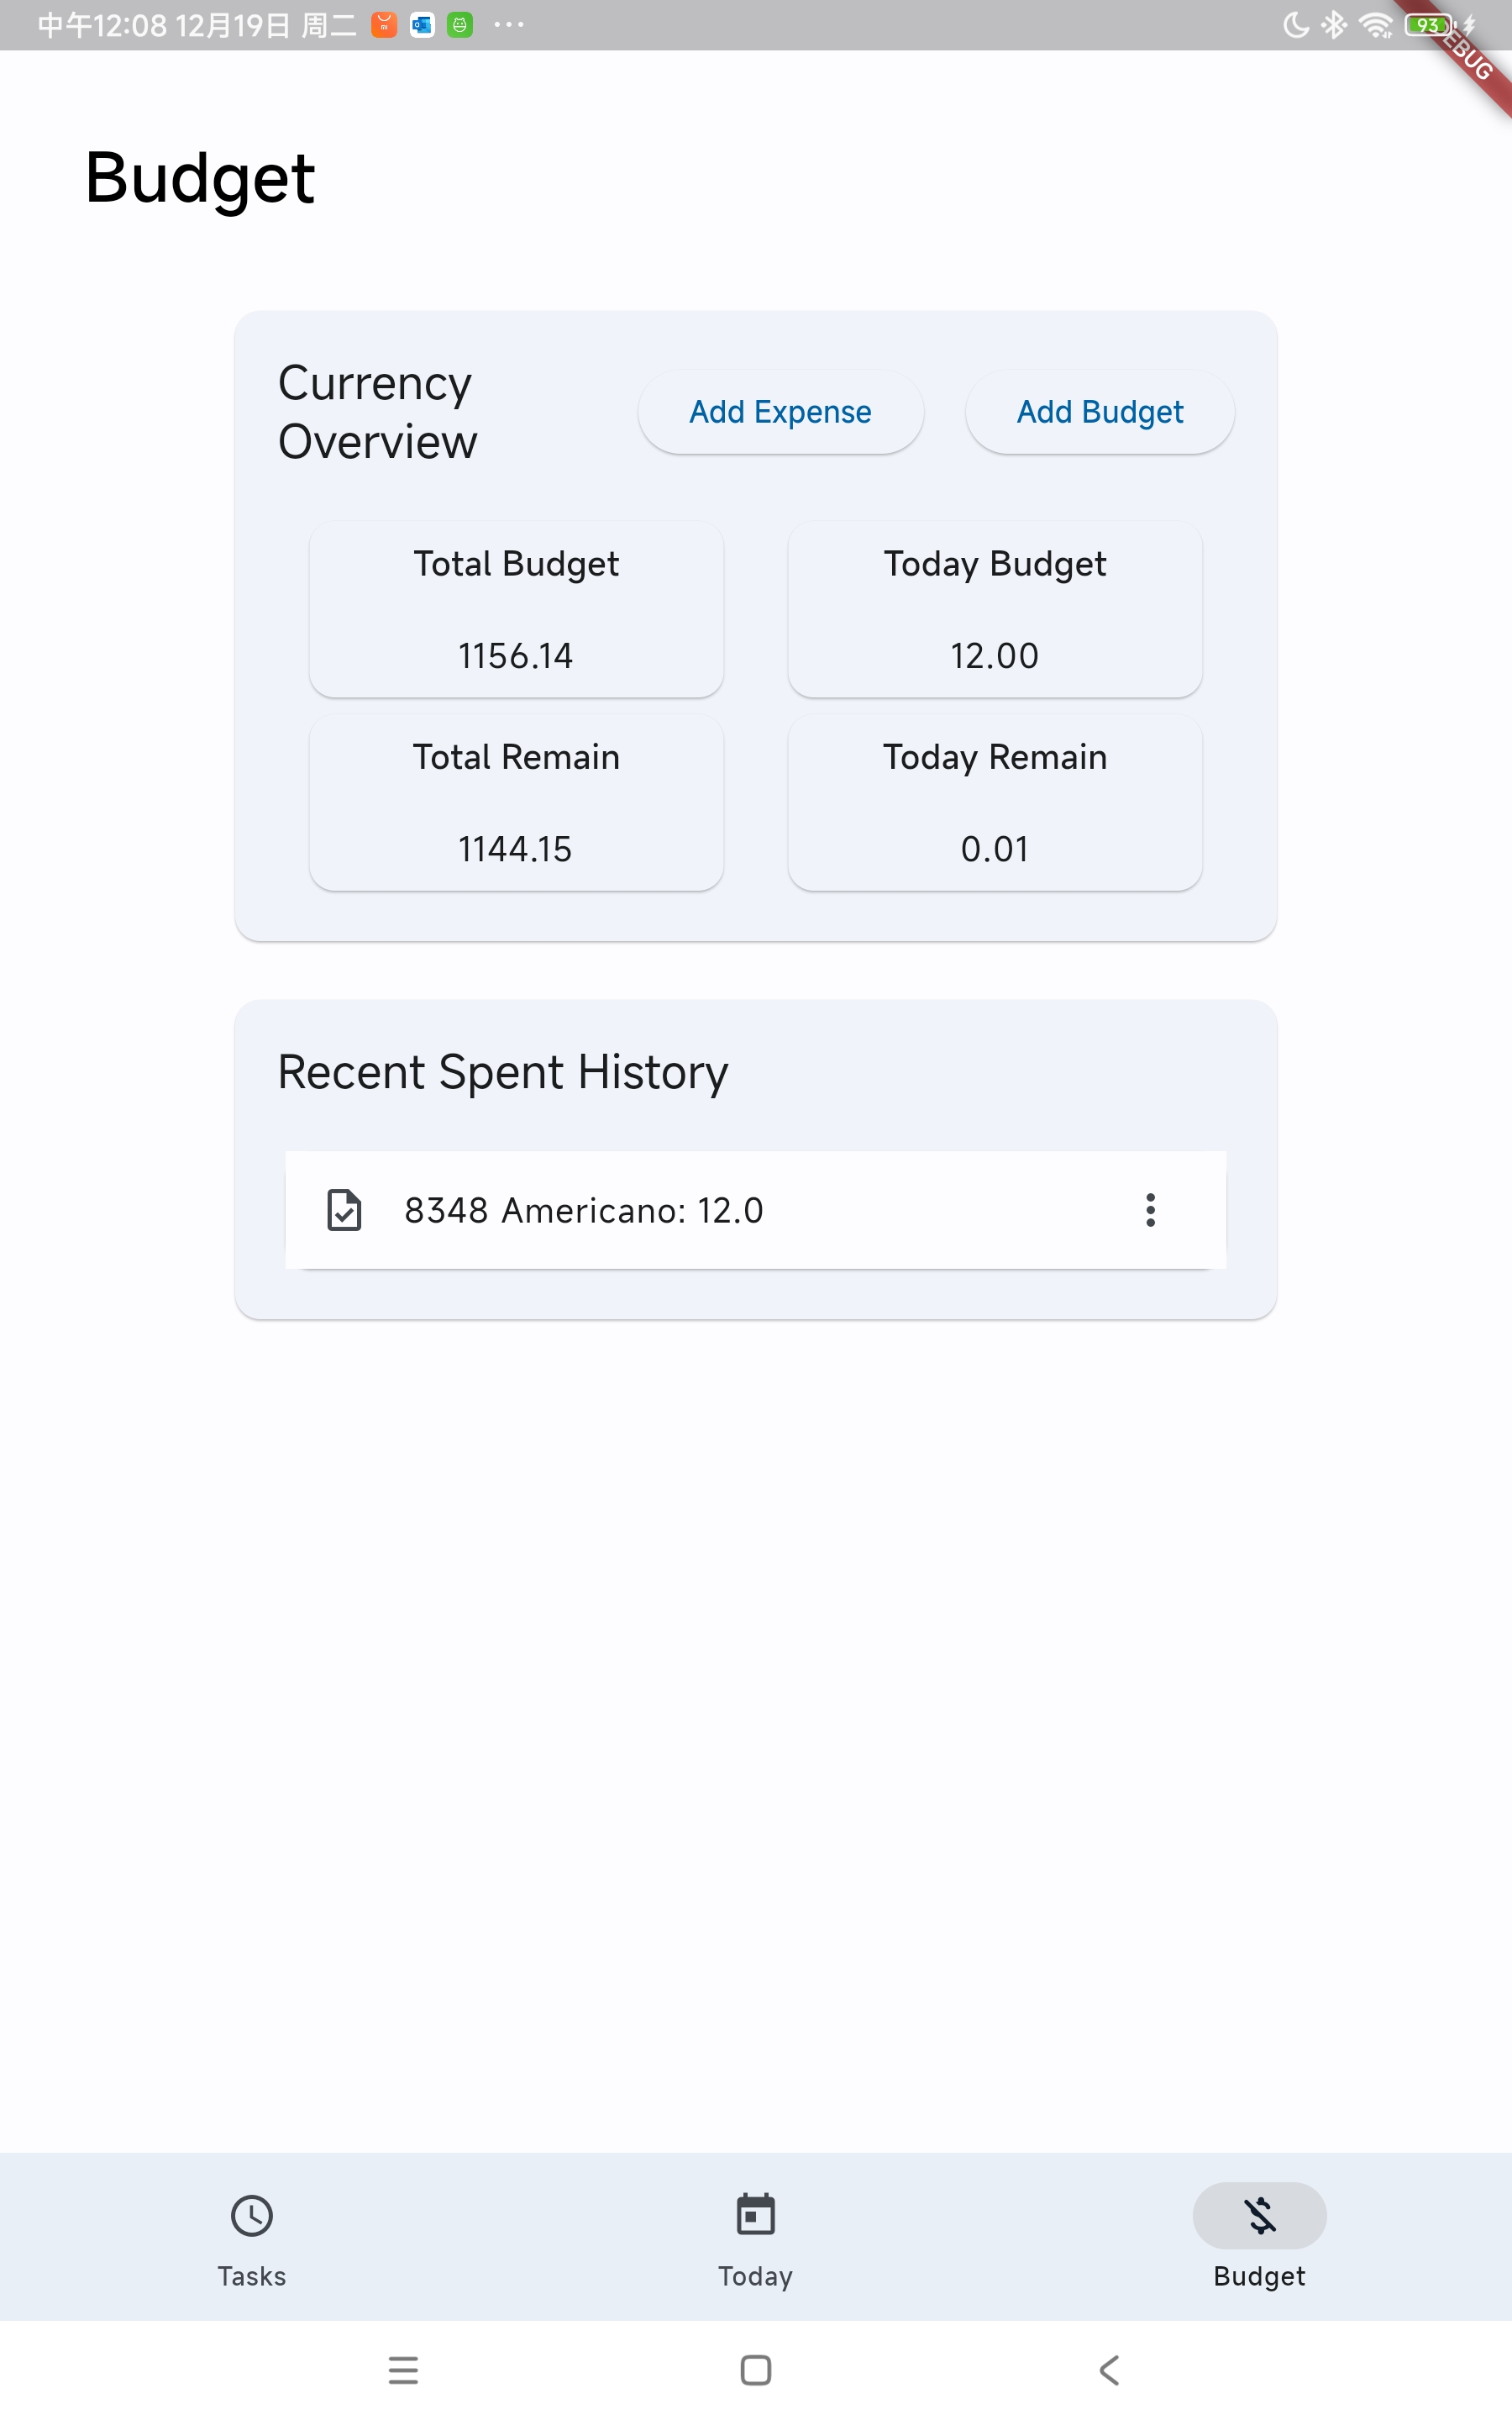
\includegraphics[width=.85\textwidth]{page-budget.jpg}
            \end{minipage}
        \end{center}
    \end{frame}

    \begin{frame}{界面预览(傳自我的手機)}
        \begin{center}
            \begin{minipage}[l]{.45\textwidth}
                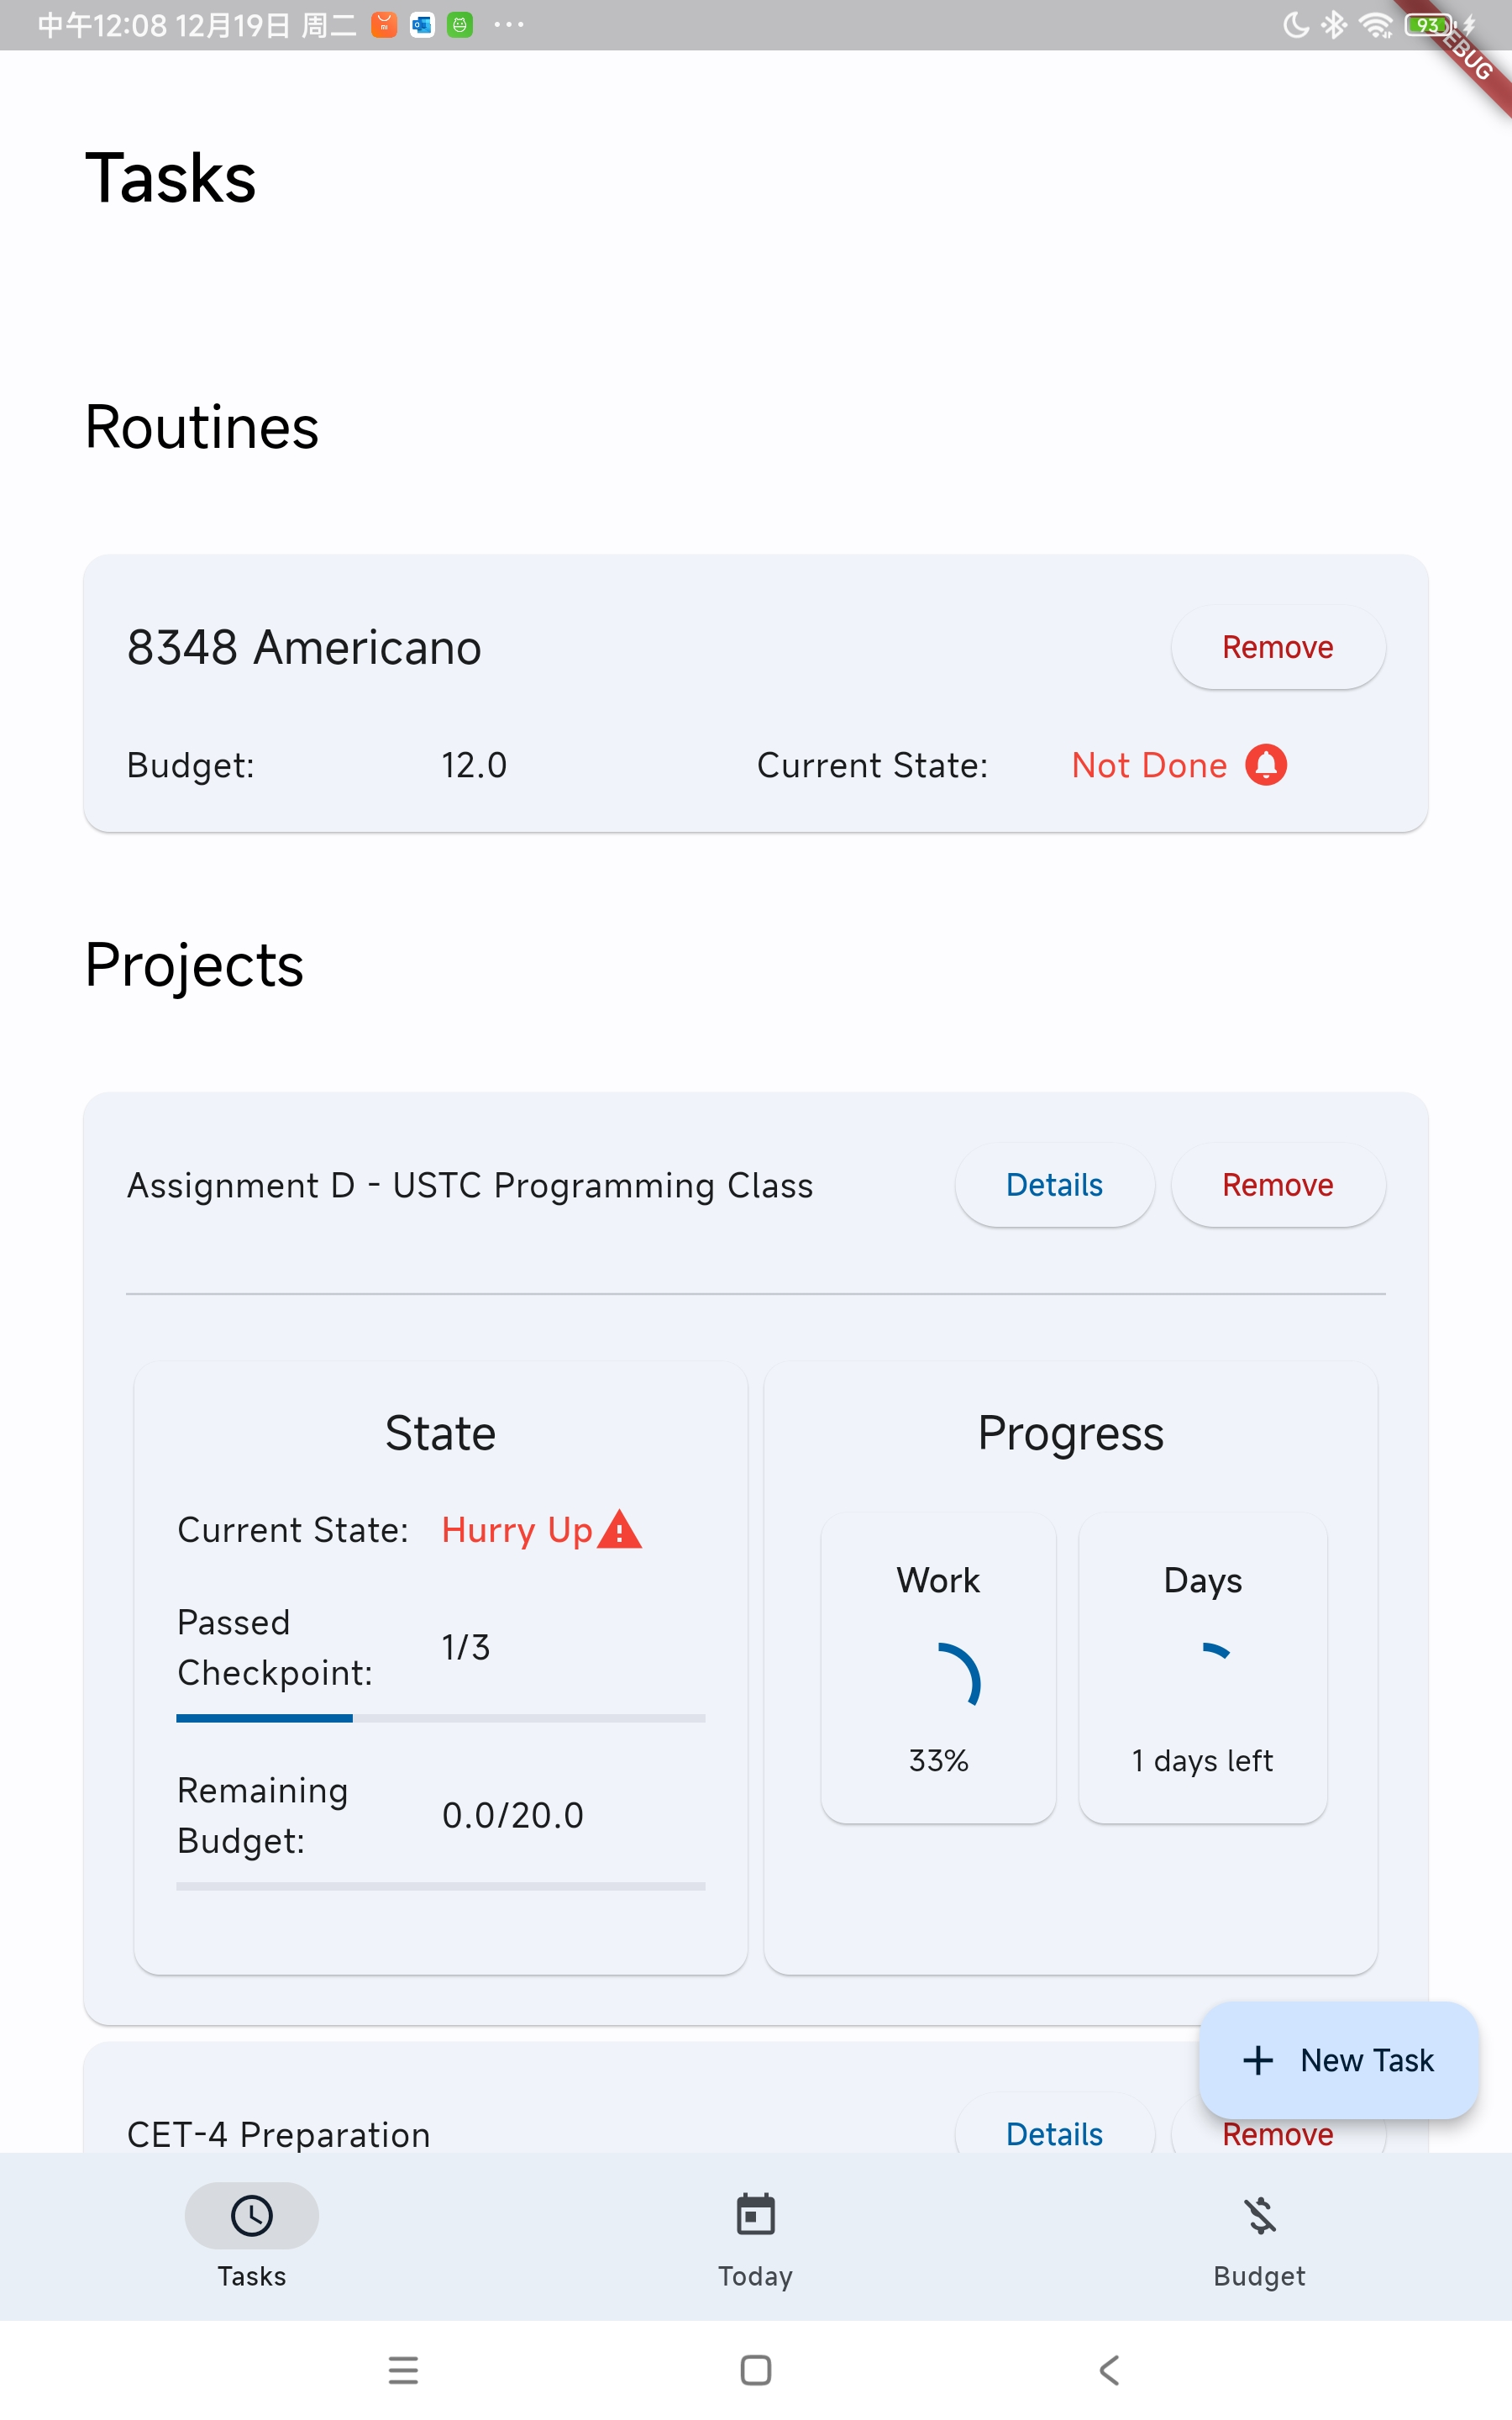
\includegraphics[width=.85\textwidth]{page-tasks.jpg}
            \end{minipage}
            \begin{minipage}[r]{.45\textwidth}
                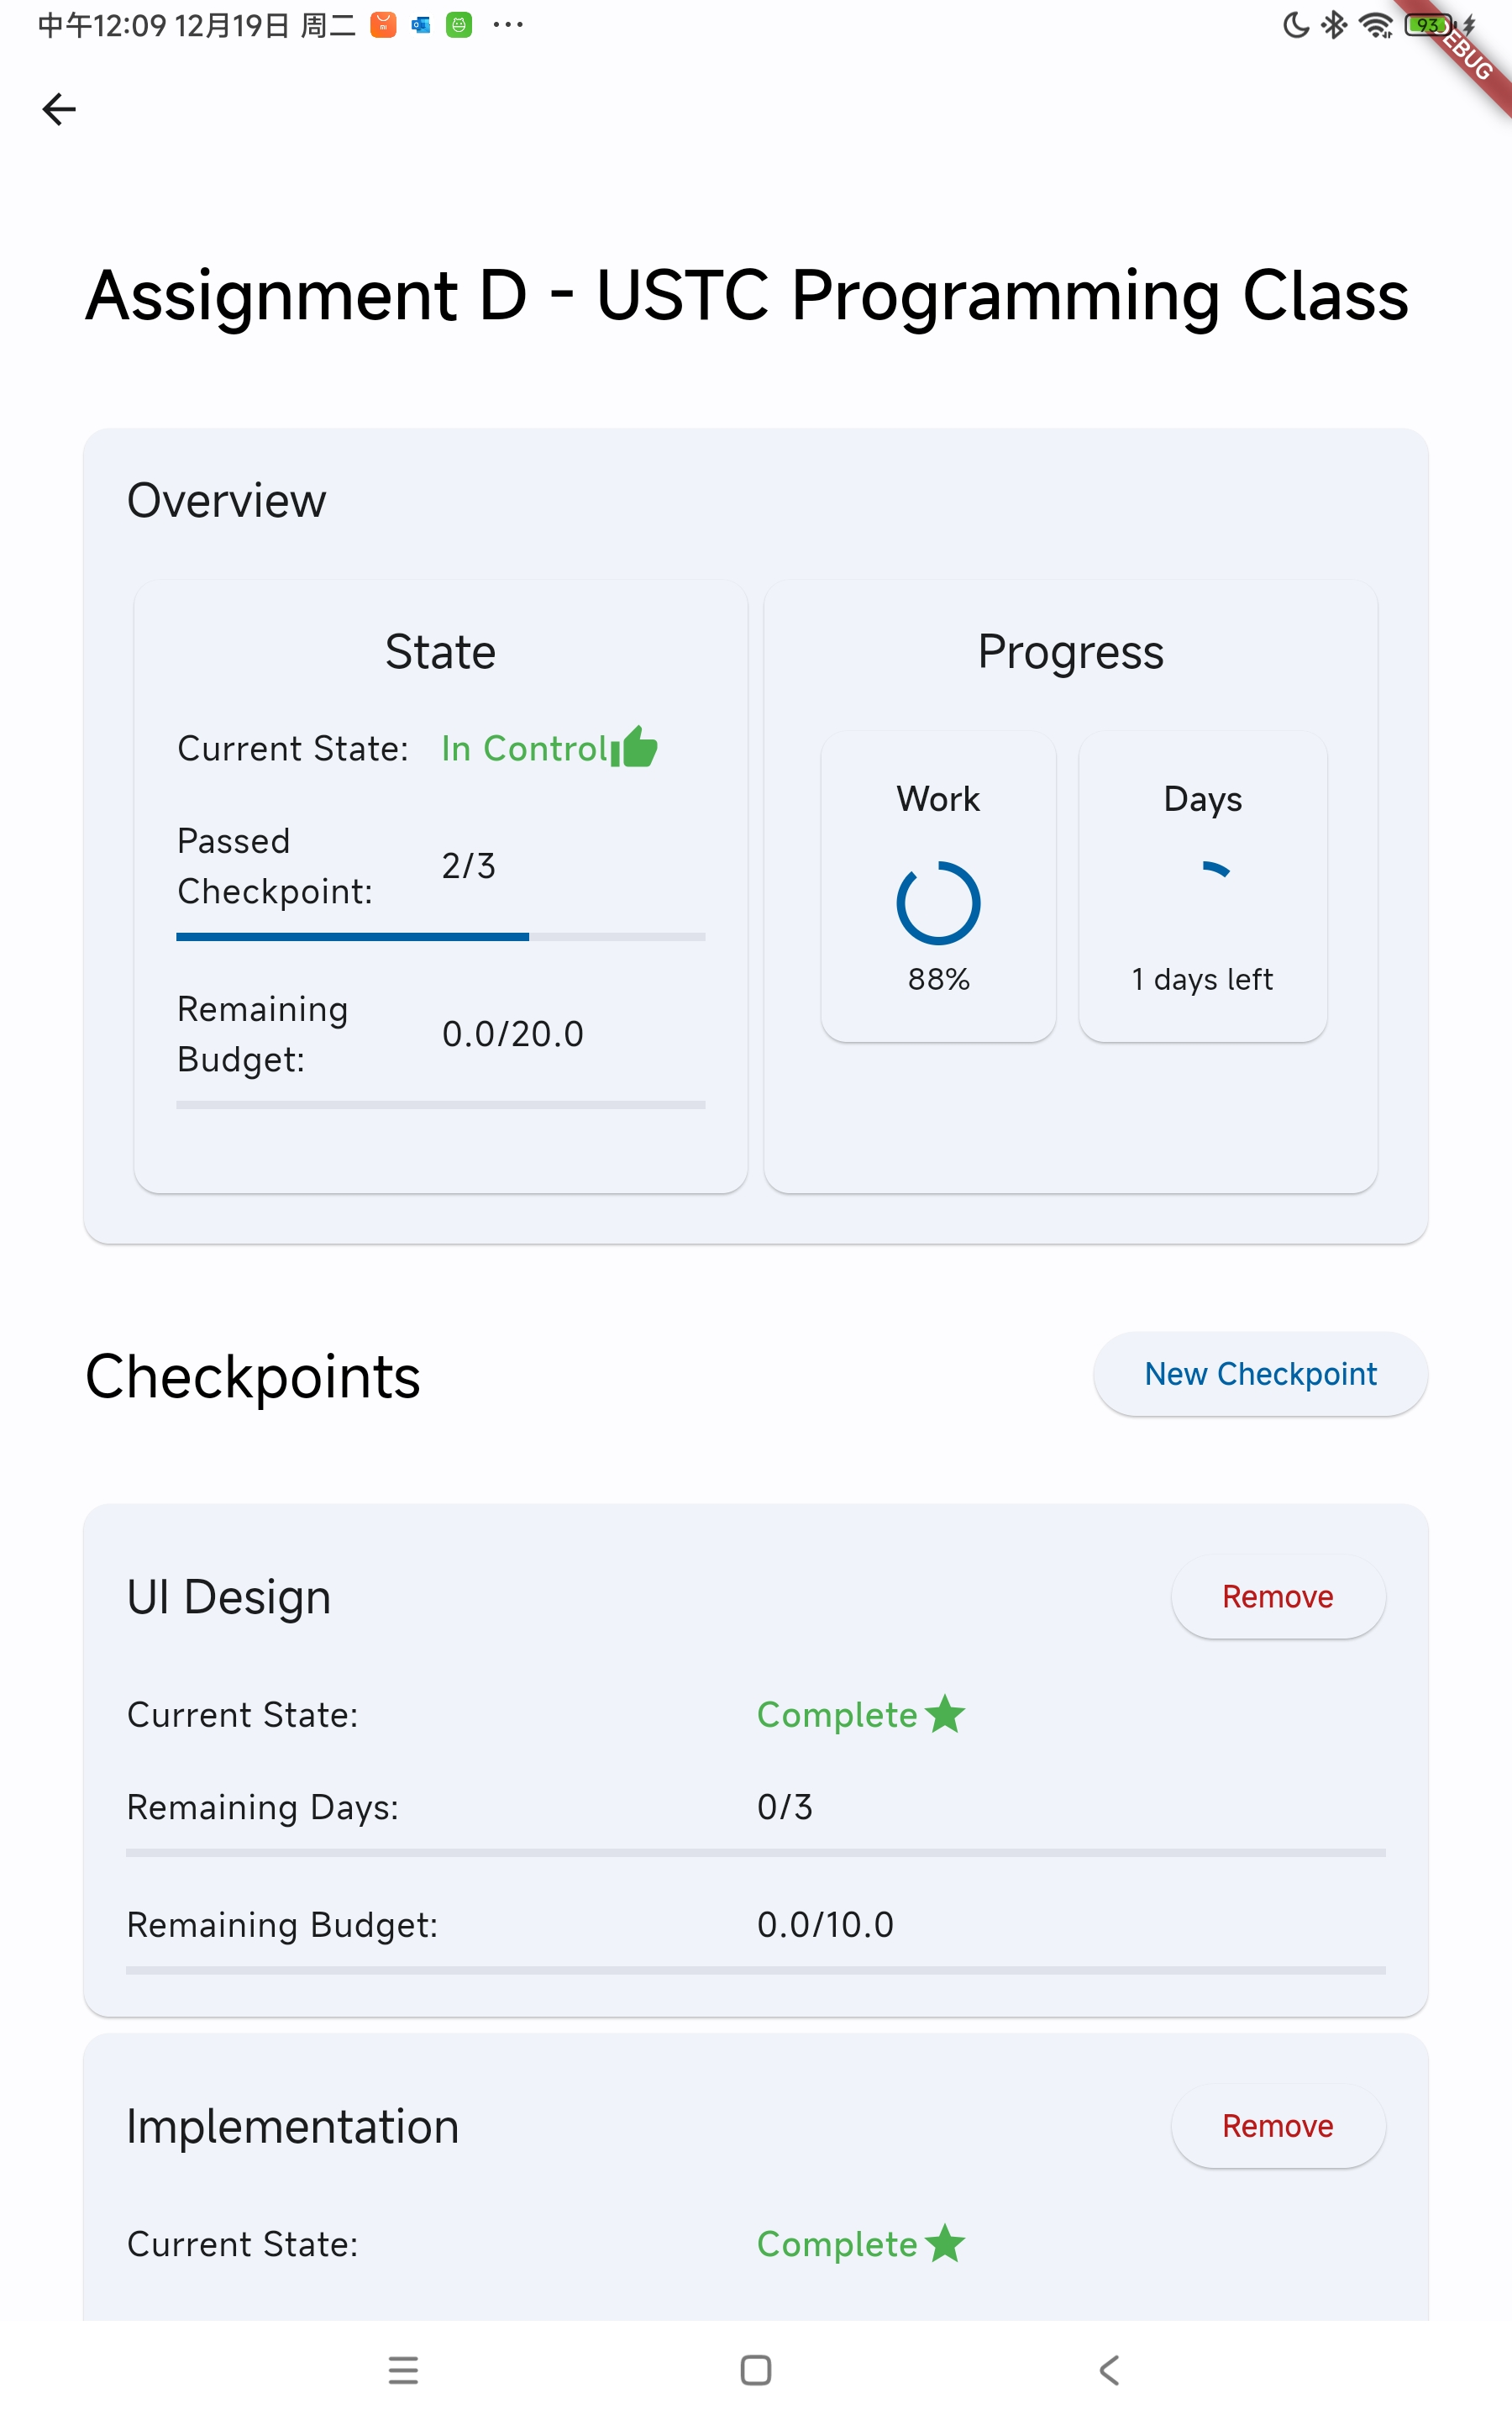
\includegraphics[width=.85\textwidth]{page-view.jpg}
            \end{minipage}
        \end{center}
    \end{frame}

    \begin{frame}{界面预览(傳自我的天選四)}
        \begin{center}
            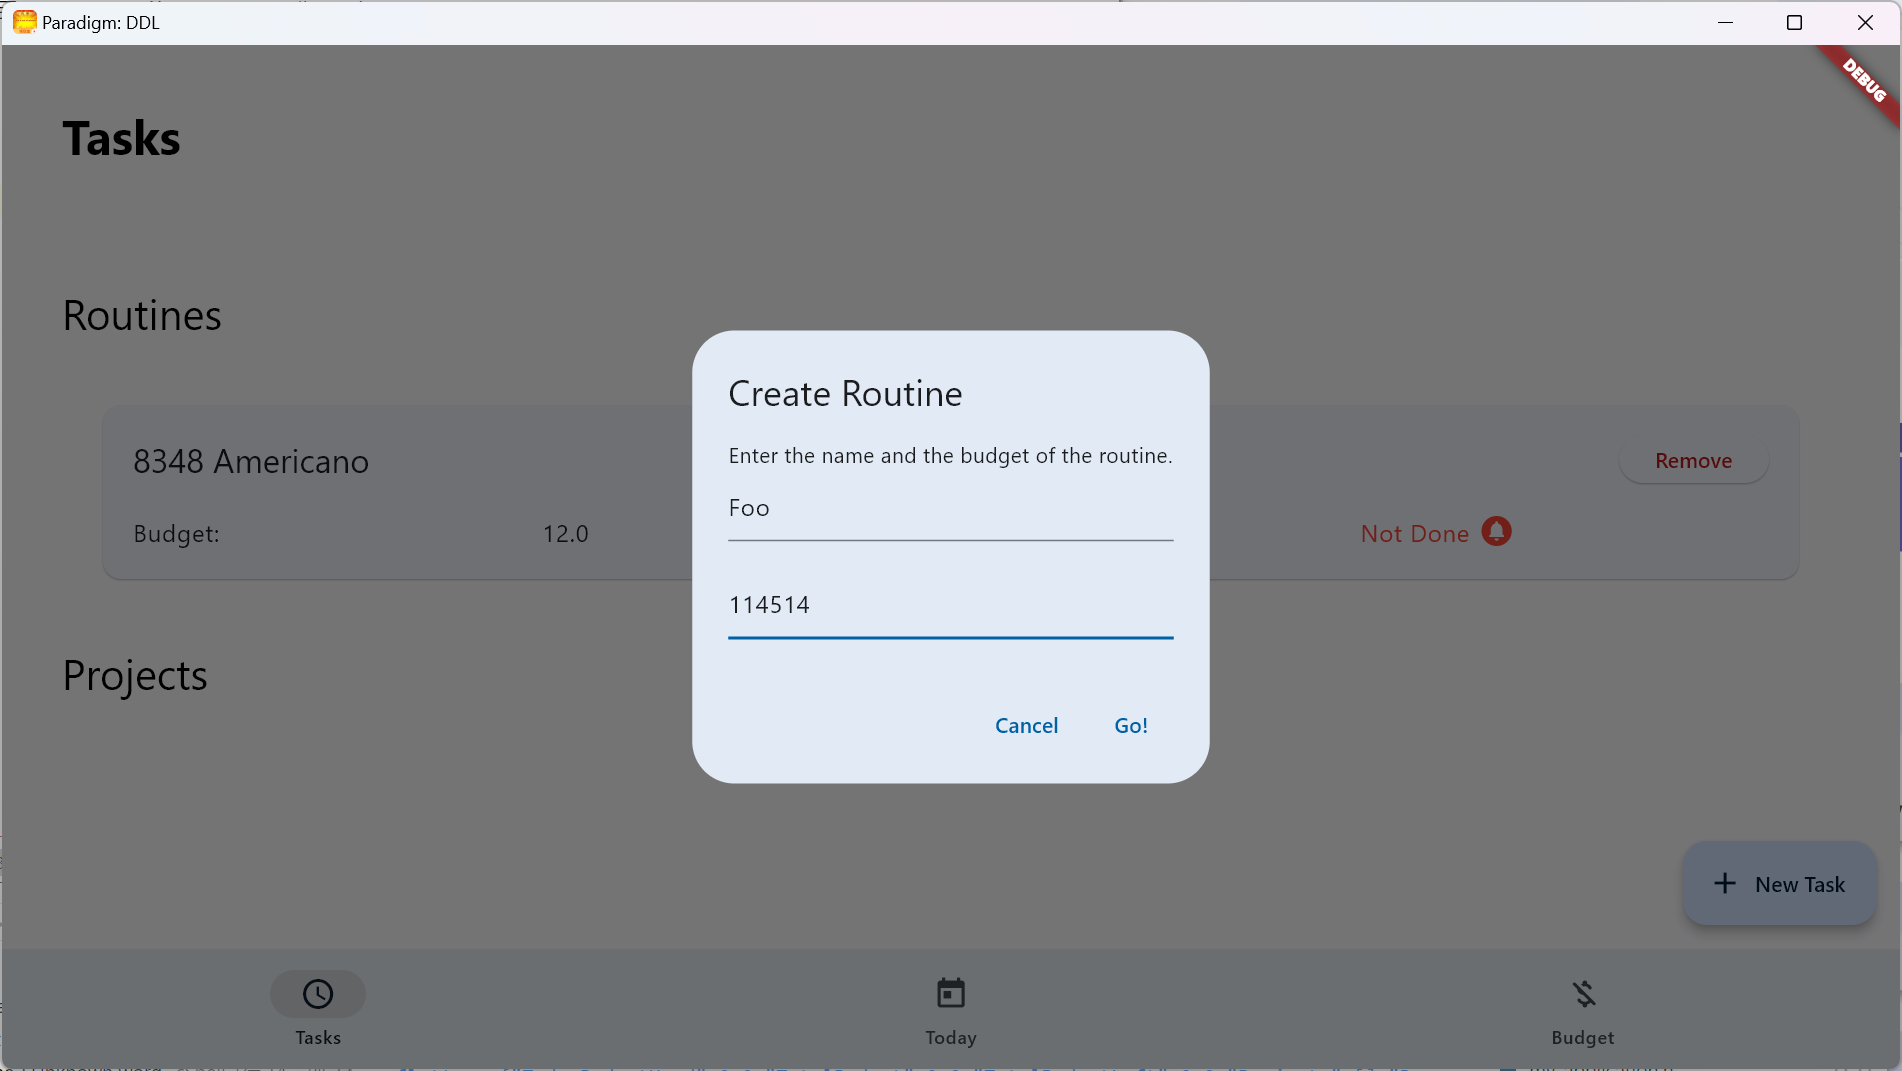
\includegraphics[width=.85\textwidth]{page-pc.png}
        \end{center}
    \end{frame}

    \begin{frame}{实机演示}
        \centering
        \Huge 实机演示
    \end{frame}

    \section{后续开发计划}

    \begin{frame}
        \sectionpage
    
        
    
    \end{frame}

    \begin{frame}
        \frametitle{后续重点计划}
        \vfill
        \begin{center}
            \begin{Huge}
                重构!
            \end{Huge}
            \vfill
            (新手一周速成的后果:未出新手村便成屎山qwq)
        \end{center}
    
    \end{frame}
	
	\begin{frame}
        \frametitle{后续功能更新}
        \vfill
        \begin{itemize}
            \item 增加i18n支持;\\\vfill
            \item 增加周常计划支持;\\\vfill
            \item 增加教务系统支持,一键导入课表/考试信息;\\\vfill
            \item 自动Checkpoint安排功能;\\\vfill
            \item 更好的输入方式;\\\vfill
            \item 基于rec网的自动/手动同步功能;\\\vfill
            \item 其他……
        \end{itemize}
    
    \end{frame}
	
	
	\begin{frame}
		\Huge{\centerline{Thank you for listening!}}
		\centering{$(*\slash\omega\backslash*)$}
	\end{frame}
	
\end{document}